%!Mode:: "TeX:UTF-8"
%!TEX program  = xelatex
\documentclass[bwprint]{cumcmthesis}
%\documentclass[withoutpreface,bwprint]{cumcmthesis} %去掉封面与编号页
\title{论文标题}
\tihao{题号}
\baominghao{报名号}
\schoolname{学校名称}
\membera{队员1}
\memberb{队员2}
\memberc{队员3}
\supervisor{指导老师}
\yearinput{年}
\monthinput{月}
\dayinput{日}
\begin{document}
 \maketitle
 \begin{abstract}
 摘要

\keywords{关键词\quad  关键词}
\end{abstract}

\section{ITEM}

引言 \cite{huwei}

\begin{itemize}
	\item item1 \cite{deng:01a}
	\item item2
	\item item3
\end{itemize}

\section{公式}

\subsection{公式1}

\[
\begin{pmatrix}{*{20}c}
{a_{11} } & {a_{12} } & {a_{13} }  \\
{a_{21} } & {a_{22} } & {a_{23} }  \\
{a_{31} } & {a_{32} } & {a_{33} }  \\
\end{pmatrix}
= \frac{{Opposite}}{{Hypotenuse}}\cos ^{ - 1} \theta \arcsin \theta
\]

\subsection{公式2}

\[
p_{j}=\begin{cases} 0,&\text{if $j$ is odd}\\
r!\,(-1)^{j/2},&\text{if $j$ is even}
\end{cases}
\]

\subsection{公式3}

\[
\arcsin \theta  =
\mathop{{\int\!\!\!\!\!\int\!\!\!\!\!\int}\mkern-31.2mu
	\bigodot}\limits_\varphi
{\mathop {\lim }\limits_{x \to \infty } \frac{{n!}}{{r!\left( {n - r}
			\right)!}}} \eqno (1)
\]

\section{表格}

\begin{tabular}{cc}
	\hline
	\makebox[0.4\textwidth][c]{C1}	&  \makebox[0.5\textwidth][c]{C2} \\ \hline
	A	    & 中文测试\\ \hline
	B	    & 中文测试 \\ \hline
	C	    & 中文测试 \\ \hline
\end{tabular}

\section{图片}

\subsection{eps}

\begin{figure}[h]
	\centering
	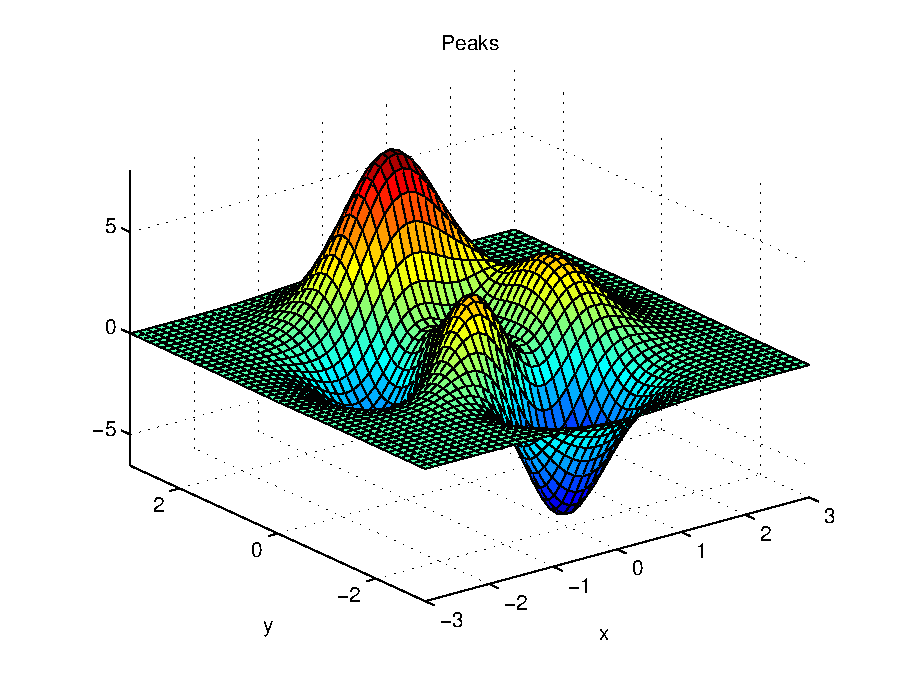
\includegraphics[width=\textwidth]{eps.eps}
	\caption{eps}
\end{figure}
\clearpage
\subsection{pdf}

\begin{figure}[h]
	\centering
	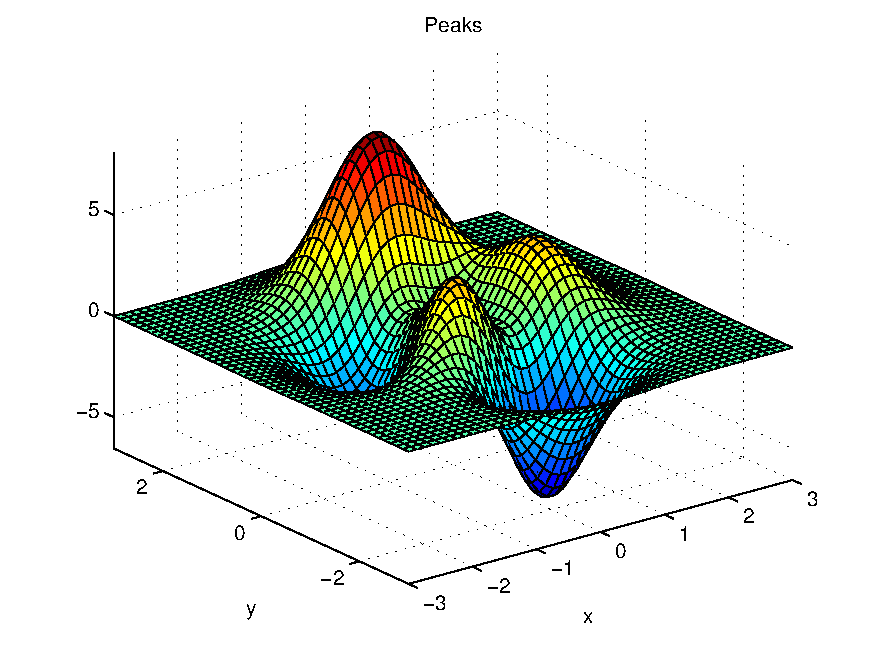
\includegraphics[width=\textwidth]{pdf.pdf}
	\caption{pdf}
\end{figure}
\clearpage
\subsection{jpg}

\begin{figure}[h]
	\small
	\centering
	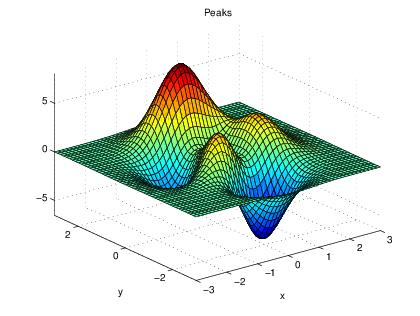
\includegraphics[width=12cm]{jpg.jpg}
	\caption{aa}
\end{figure}
\clearpage

%参考文献
\bibliographystyle{plain}
\nocite{*}
\bibliography{reference}

\newpage
%附录
\appendix
\section{Matlab程序}

\textcolor[rgb]{0.98,0.00,0.00}{\textbf{matlab.m:}}

\lstinputlisting[language=Matlab]{code/matlab.m}

\section{C++程序}

\textcolor[rgb]{0.98,0.00,0.00}{\textbf{cpp.cpp:}}

\lstinputlisting[language=C++]{code/cpp.cpp}

\end{document} 